\chapter{Methodology}
\label{ch:methodology}

\section{Introduction}
This chapter explains the approach, methods and techniques used to build the proposed system. The work followed a service-based approach in which the system was divided into four applications with clear responsibilities, and the business modules were built on a shared foundation of authentication, permissions and institution-level data separation. Each module was developed together with automated tests that exercise it through its real HTTP interface and database.

The chapter first describes the overall development approach and how the applications are organised. It then explains the method used to authenticate and authorise every request and keep institutions' data apart. The following sections present the techniques behind the intelligent parts of the system: the machine learning models used for student risk and GPA prediction, together with the synthetic data on which they are trained; the text processing, retrieval and ranking method used by the message assistant to find trusted answers; the method used to forward unanswered questions to staff and review their answers; and the speech processing method used for voice calls. The final section describes the testing approach used to check the system.

\section{Development Approach}
The system is divided into four independently runnable applications. The Next.js frontend contains only the user interface and talks to nothing but the Core API. The Core API holds all business rules and is the single gateway to the database and to the other services. The AI service performs machine learning prediction, and the Voice service performs language and speech processing. This division keeps each technology where it fits best: TypeScript and Express for transactional business logic, and Python for machine learning, language models and speech, which depend on Python libraries.

Inside the Core API, each business area is a module with the same structure: a controller that declares the HTTP routes and the permission each route needs, services that apply the business rules inside database transactions, and, for larger areas such as the hostel, repositories that contain the SQL queries. All modules share common middleware for request context, authentication and error handling, and all tables are defined in one database schema file that is applied when the database is created. Configuration such as database addresses, secrets, model names and provider settings is read from environment variables, so the same code runs on a developer's machine and in containers.

All business modules, such as academics, finance, hostel, library, human resources, inventory, notices and the assistant, are built on a shared foundation of identity, roles, permissions and institution separation, so a new module only adds its own routes, tables and rules, together with its own automated tests. Work that must happen without a user, such as generating invoices, sending reminders or processing uploaded documents, was placed in background schedulers inside the Core API. Each scheduled job can be repeated safely, catches up after downtime, and takes a database advisory lock so that two running servers never perform the same job at the same time.

\section{Authentication, Authorisation and Data Isolation}
Every request to the Core API passes through the same sequence of checks before it reaches a module. The method is shown in Algorithm~\ref{alg:auth}. Requests from the AI and Voice services are recognised by a shared service token and act for the institution named in the request. Requests from users must carry a valid signed JSON Web Token. The token only identifies the user; the user's current account status, role, permissions and institution status are read from the database on every request, so a change made by an administrator takes effect on the very next request rather than when the token expires.

\begin{algorithm}
    \caption{Authenticating and authorising a Core API request}
    \label{alg:auth}
    \begin{algorithmic}[1]
    \State Receive request $r$ for route $p$ with required permission $k$
    \If{$p$ is a public route (health, sign-in, public hostel payment, registration, assistant reply link)}
        \State Pass $r$ to the module
    \ElsIf{$r$ carries a valid service token from the AI or Voice service}
        \State Treat $r$ as an internal service call for the institution named in $r$
    \ElsIf{$r$ has no valid signed JSON Web Token}
        \State \Return 401 Unauthorized
    \Else
        \State Load user $u$, role, permissions and institution status from the database
        \If{$u$ is disabled or the institution is not active}
            \State \Return 403 Forbidden
        \EndIf
        \If{$u$ must change a temporary password}
            \State \Return 403 Password change required
        \EndIf
        \If{$k \notin$ permissions of $u$}
            \State \Return 403 Forbidden
        \EndIf
        \State Pass $r$ to the module with the institution of $u$
    \EndIf
    \State The module limits every query to the institution of the request
    \end{algorithmic}
\end{algorithm}

Passwords are stored as bcrypt hashes. When a user signs in, the system counts consecutive failures; on the fifth failure the account is locked for fifteen minutes, and both failed and successful sign-ins are written to the audit log. A user who signs in with a temporary password receives a token that is valid for only fifteen minutes and can do nothing except choose a new password; other tokens are valid for eight hours. Data isolation is achieved by storing an institution identifier on every record and adding it to the condition of every query. The Voice service, which writes call transcripts directly, uses its own database login whose access to the transcript tables is restricted by PostgreSQL row security policies.

\section{Student Risk and GPA Prediction}
The AI service provides two prediction models, shown in Figure~\ref{fig:prediction}. Both are trained when the service starts. Because the project did not have access to real student records, both models are trained on synthetic data generated with a fixed random seed of 42, so that results are repeatable. The aim of this method is to demonstrate how prediction fits into the platform; the models are not validated on real data.

\begin{figure}[htbp]
  \centering
  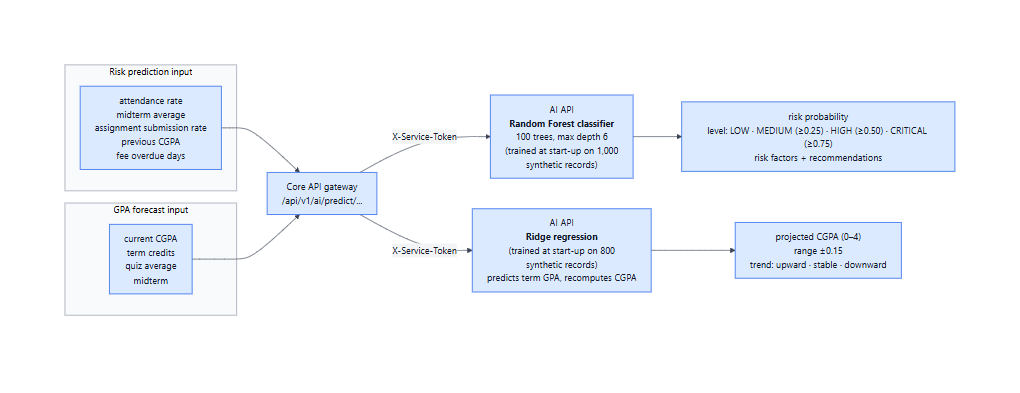
\includegraphics[width=\textwidth,height=0.85\textheight,keepaspectratio]{book_figures/fig11_ai_prediction.png}
  \caption{Student risk prediction and GPA forecast models}
  \label{fig:prediction}
\end{figure}

\subsection{Academic risk classifier}
The risk model uses five input features: attendance rate $A$ (percent), midterm average $M$ (out of 100), assignment submission rate $S$ (percent), previous CGPA $C$ (out of 4, scaled to $25C$) and days of overdue fees $F$. For training, 1,000 synthetic students are generated with $A \sim U(40,100)$, $M \sim U(30,100)$, $S \sim U(20,100)$, $25C \sim U(35,100)$ and $F \sim \mathrm{Exp}(10)$. Each synthetic student is labelled at risk ($y=1$) or in good standing ($y=0$) by the scoring rule in Equations~\ref{eq:risk-logit} and~\ref{eq:risk-label}:

\begin{equation} \label{eq:risk-logit}
    z = -0.04A - 0.03M - 0.02S - 0.03(25C) + 0.02F + 7.5
\end{equation}

\begin{equation} \label{eq:risk-label}
    y = \begin{cases} 1 & \text{if } \dfrac{1}{1+e^{-z}} > 0.5 \\ 0 & \text{otherwise} \end{cases}
\end{equation}

The features are standardised, and a Random Forest classifier with 100 trees and a maximum depth of 6 is trained on the labelled data. For a new student with feature vector $\mathbf{x}$, the risk probability is the average of the probabilities given by the $T=100$ trees:

\begin{equation} \label{eq:rf}
    P(\text{risk} \mid \mathbf{x}) = \frac{1}{T}\sum_{t=1}^{T} P_t(\text{risk} \mid \mathbf{x})
\end{equation}

The probability is turned into a risk level using the thresholds in Table~\ref{tab:risk-levels}. Independently of the model, the service checks each input against a fixed threshold and, when it is crossed, reports the reason and a recommended action for staff, as listed in Table~\ref{tab:risk-factors}.

\begin{table}[H]
    \centering
        \caption{Risk levels from the predicted probability}
        \label{tab:risk-levels}
        \begin{tabular}{|c|c|}
        \hline
        \textbf{Risk probability} & \textbf{Risk level}\\
        \hline
        $P \geq 0.75$ & Critical \\
        \hline
        $0.50 \leq P < 0.75$ & High \\
        \hline
        $0.25 \leq P < 0.50$ & Medium \\
        \hline
        $P < 0.25$ & Low \\
        \hline
        \end{tabular}
\end{table}

\begin{table}[H]
    \centering
        \caption{Risk factors and recommended actions}
        \label{tab:risk-factors}
        \begin{tabular}{|p{4.2cm}|p{8.8cm}|}
        \hline
        \textbf{Condition} & \textbf{Recommended action}\\
        \hline
        Attendance below 75\% & Assign an academic advisor consultation for attendance \\
        \hline
        Midterm average below 50 & Schedule remedial tutorial sessions for core examination topics \\
        \hline
        Assignment submission below 60\% & Send automated assignment deadline reminders \\
        \hline
        CGPA below 2.50 & Limit extra-curricular registrations and audit the course load \\
        \hline
        Fees overdue more than 30 days & Connect the student with the financial welfare board for a scholarship or installment plan \\
        \hline
        \end{tabular}
\end{table}

\subsection{GPA forecast model}
The GPA model predicts a student's term GPA from the current CGPA $C$, the quiz average $Q$ and the midterm marks $M$. For training, 800 synthetic records are generated with $C \sim U(2,4)$, $Q \sim U(40,100)$ and $M \sim U(40,100)$, and the term GPA $g$ is computed by Equation~\ref{eq:gpa-synth}, where $\varepsilon \sim N(0, 0.15)$ and the result is limited to the range 0 to 4:

\begin{equation} \label{eq:gpa-synth}
    g = 0.30\,C + 0.015\,Q + 0.020\,M + \varepsilon
\end{equation}

A ridge regression model is fitted to these records. Ridge regression chooses the coefficient vector $\mathbf{w}$ that minimises the squared error plus a penalty on the size of the coefficients, with $\alpha = 1$:

\begin{equation} \label{eq:ridge}
    \hat{\mathbf{w}} = \arg\min_{\mathbf{w}} \; \lVert \mathbf{y} - X\mathbf{w} \rVert^2 + \alpha \lVert \mathbf{w} \rVert^2
\end{equation}

The predicted term GPA $\hat{g}$ is limited to the range 0 to 4 and combined with the current CGPA, assuming 45 previously completed credits, to give the projected CGPA for a term of $c$ credits:

\begin{equation} \label{eq:cgpa}
    \text{CGPA}_{\text{new}} = \frac{45\,C + c\,\hat{g}}{45 + c}
\end{equation}

The service returns the projected CGPA with a range of $\pm 0.15$, and describes the trend as upward if the projection is more than 0.05 above the current CGPA, downward if it is more than 0.05 below, and stable otherwise.

\section{Knowledge Retrieval and Answer Selection}
The message assistant must answer only from trusted sources. Its method has three parts: deciding what kind of question has been asked, finding and ranking relevant passages, and choosing how, or whether, to answer. The overall flow is shown in Figure~\ref{fig:assistant}.

\begin{figure}[htbp]
  \centering
  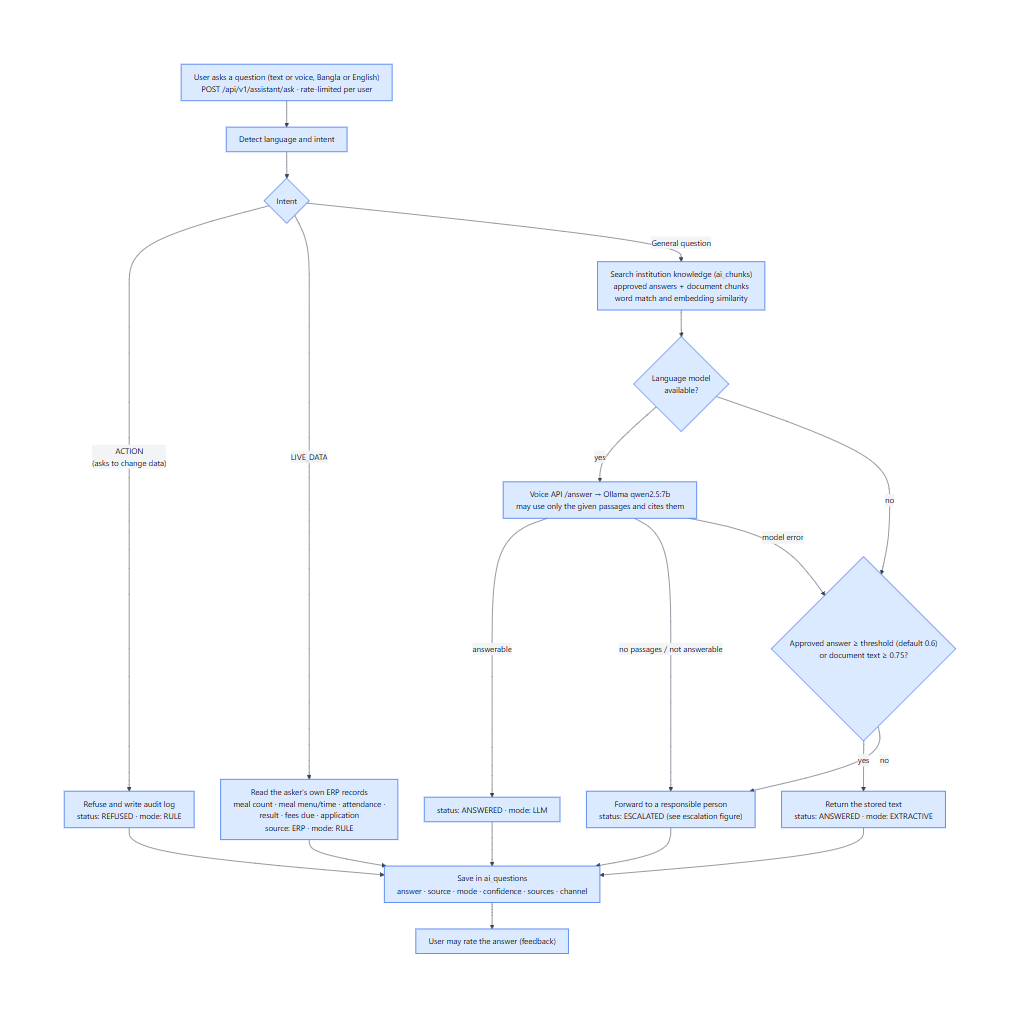
\includegraphics[width=\textwidth,height=0.85\textheight,keepaspectratio]{book_figures/fig07_assistant_answer_flow.png}
  \caption{Message assistant question answering flow}
  \label{fig:assistant}
\end{figure}

\subsection{Language and intent detection}
A question is treated as Bangla if it contains any character from the Bangla Unicode block, and as English otherwise; the answer is given in the same language. Each user may ask up to 20 questions per minute. The intent is then decided by pattern rules in a fixed order, as listed in Table~\ref{tab:intents}.

\begin{table}[H]
    \centering
        \caption{Question intents and how they are answered}
        \label{tab:intents}
        \begin{tabular}{|p{2.6cm}|p{5.2cm}|p{5.2cm}|}
        \hline
        \textbf{Intent} & \textbf{Detected when} & \textbf{Answered by}\\
        \hline
        Action & The question asks to change, delete, create, approve, pay or similar, in English, Bangla or Bangla written in English letters & A polite refusal, recorded in the audit log \\
        \hline
        Live data & The question matches a topic pattern: meal count, meal menu, meal time or fees due; or attendance, result or application when the question also refers to the asker & The asker's own records in the database \\
        \hline
        Knowledge & Any other question & Retrieval from documents and approved answers \\
        \hline
        \end{tabular}
\end{table}

\subsection{Text processing and chunking}
Documents uploaded by administrators are read as text and split into chunks. Paragraphs of up to 900 characters form one chunk; longer paragraphs are split at sentence ends into chunks of about 900 characters, with an overlap of 150 characters so that a sentence near a boundary is not lost. Questions, chunks and approved answers are reduced to search terms by normalising Unicode, converting to lower case, splitting on any character that is not a letter, digit or combining mark, removing English and Bangla stop words, and applying a simple stemmer. When an embedding model is available, each chunk is also given a bge-m3 embedding vector. Approved answers are stored as chunks in the same way, so documents and approved answers are searched together.

\subsection{Ranking}
Each candidate chunk shares at least one term with the question or, when embeddings are available, is compared with the question by meaning. Let $N$ be the number of active chunks of the institution and $n_t$ the number of chunks that contain term $t$. The importance of a term is its inverse document frequency:

\begin{equation} \label{eq:idf}
    \mathrm{idf}(t) = \ln\!\left(1 + \frac{N - n_t + 0.5}{n_t + 0.5}\right)
\end{equation}

For a question with term set $Q$ and a chunk $d$ that contains the matched terms $Q_d \subseteq Q$, the system computes the BM25 relevance score with $k_1 = 1.2$, $b = 0.75$ and an average chunk length of 150 words, where $f_t$ is the number of times $t$ appears in $d$ and $|d|$ is the number of words in $d$:

\begin{equation} \label{eq:bm25}
    \mathrm{BM25}(d) = \sum_{t \in Q_d} \mathrm{idf}(t)\,\frac{f_t\,(k_1 + 1)}{f_t + k_1\left(1 - b + b\,\frac{|d|}{150}\right)}
\end{equation}

It also computes the coverage, the share of the question's importance that the chunk contains, using $W(T) = \sum_{t \in T} \mathrm{idf}(t)$:

\begin{equation} \label{eq:coverage}
    \mathrm{cov}(d) = \frac{W(Q_d)}{W(Q)}
\end{equation}

For an approved answer, whose original question has term set $K$, the similarity between the two questions is the harmonic mean of how much of the new question is covered and how much of the stored question is covered:

\begin{equation} \label{eq:similarity}
    \mathrm{sim} = \frac{2\,f\,g}{f + g}, \qquad f = \frac{W(Q \cap K)}{W(Q)}, \quad g = \frac{W(Q \cap K)}{W(K)}
\end{equation}

The word-based score $L$ is the coverage for a document chunk and $\max(\mathrm{sim}, 0.9\,\mathrm{cov})$ for an approved answer. When embeddings are available, the meaning-based score is the cosine similarity $s$ between the question vector and the chunk vector, and the final score combines both:

\begin{equation} \label{eq:score}
    \mathrm{score}(d) = \begin{cases} L + \dfrac{\mathrm{BM25}(d)}{100} & \text{without embeddings} \\[2ex] 0.5\,L + 0.5\,\max(0, s) + \dfrac{\mathrm{BM25}(d)}{100} & \text{with embeddings} \end{cases}
\end{equation}

A chunk is kept only if $L > 0$ or $s \geq 0.5$, and the six chunks with the highest scores are returned.

\subsection{Answer selection}
The ranked chunks are used as described in Algorithm~\ref{alg:answer}. With the language model, only passages that share enough words with the question or are close enough in meaning are given to the model, and the model must answer only from them and report which passages it used. Without the language model, the assistant returns stored text only when the match is strong; the confidence threshold $\theta$ is set by each institution and defaults to 0.6.

\begin{algorithm}
    \caption{Choosing the answer to a knowledge question}
    \label{alg:answer}
    \begin{algorithmic}[1]
    \State Retrieve the top six ranked chunks $H$ for question $q$
    \If{the language model is available}
        \State $P \gets \{h \in H : \max(\mathrm{cov}_h, \mathrm{sim}_h) \geq 0.2 \text{ or } s_h \geq 0.55\}$
        \If{$P = \emptyset$}
            \State \Return forward $q$ to a responsible person
        \EndIf
        \State Ask qwen2.5:7b to answer $q$ using only $P$ and to list the passages used
        \If{the model answers}
            \State \Return the answer with its cited passages (mode: LLM)
        \ElsIf{the model says $P$ does not answer $q$}
            \State \Return forward $q$ to a responsible person
        \EndIf
        \State \Comment{If the model fails, continue without it}
    \EndIf
    \State $a \gets$ the approved answer in $H$ with the highest similarity
    \If{$a$ exists and $\max(\mathrm{sim}_a, s_a) \geq \theta$}
        \State \Return the approved answer (mode: extractive)
    \EndIf
    \State $d \gets$ the document chunk in $H$ with the highest coverage
    \If{$d$ exists and $\max(\mathrm{cov}_d, s_d) \geq \max(0.75, \theta)$}
        \State \Return the sentences of $d$ that contain the question's terms (mode: extractive)
    \EndIf
    \State \Return forward $q$ to a responsible person
    \end{algorithmic}
\end{algorithm}

\section{Question Escalation and Human Review}
A question that cannot be answered from trusted sources is forwarded rather than guessed. The responsible person is chosen by matching the question with the topics of each configured contact; if no contact's topics match, the default contact is used, and if there is none, the question waits for an administrator. The question is sent on every channel that the person uses, which may be SMS, email, a call or the person's own panel, together with a private reply link that is valid for fourteen days. A channel that is not configured or has no address is skipped. If delivery fails on a channel, it is retried later by the assistant scheduler, which runs every 30 seconds by default. After the $n$-th attempt, the next attempt is scheduled after a delay that doubles each time:

\begin{equation} \label{eq:retry}
    \Delta t_n = 2^{n} \text{ minutes}, \qquad n = 1, 2, \ldots, 4
\end{equation}

After five attempts, or if no channel can reach the person, the question is handed to an administrator. When the person answers, the reply is placed in a review queue together with a version drafted by the language model from the question and the reply. An administrator can edit, approve or reject it. Only an approved answer is stored as knowledge, indexed for search, and shown to the person who asked; from then on, similar questions can be answered from it. This human review step is what prevents unverified answers from entering the assistant's knowledge.

\section{Speech Processing}
Voice calls reuse the same answering method as typed questions, with speech recognition before it and speech synthesis after it. The browser records the caller's speech, up to 60 seconds per turn, and sends it to the Core API, which passes it to the Voice service. Speech recognition uses faster-whisper, running on the processor with 8-bit integer computation and voice activity detection to skip silence. If the caller has not chosen a language, the small Whisper model first detects whether the speech is Bangla or English. English speech is then transcribed with the small model, and Bangla speech with the large-v3-turbo model, because the small and medium models cannot read Bangla.

The transcribed text is answered by the Core API exactly as a typed question, with the channel recorded as voice. The answer text is converted to speech with the MMS text-to-speech voice of the same language, facebook/mms-tts-ben for Bangla or facebook/mms-tts-eng for English, after numbers in the text have been written out as words so that they are read correctly. Only one speech job runs at a time. Each caller and assistant turn is stored with its text, language, audio length and processing time. If speech synthesis fails, the caller still receives the written answer.

\section{Testing Approach}
The system was checked with automated tests written for each application. The Core API tests use the built-in Node.js test runner and start the real application against a PostgreSQL database; they create a temporary institution with its own users, call the HTTP endpoints as different roles, check the responses and the stored data, and remove the institution afterwards. External services such as email, SMS and the bKash gateway are replaced by fake implementations during these tests, so no real messages or payments are sent. The AI and Voice service tests use pytest. Table~\ref{tab:tests} lists the test suites and the number of test cases in each; the results of running them are reported in Chapter~VII.

\begin{table}[H]
    \centering
        \caption{Automated test suites}
        \label{tab:tests}
        \begin{tabular}{|p{3.2cm}|p{5.4cm}|c|}
        \hline
        \textbf{Application} & \textbf{Test suite} & \textbf{Test cases}\\
        \hline
        Core API & Identity and user management & 16 \\
        \hline
        Core API & Academics and general API & 8 \\
        \hline
        Core API & Hostel (rooms, rent, operations, online payment, extras) & 68 \\
        \hline
        Core API & Inventory and purchasing & 15 \\
        \hline
        Core API & Assistant and voice calls & 11 \\
        \hline
        Core API & Operations and remaining modules & 10 \\
        \hline
        AI service & Prediction, question answering and objection classifier & 5 \\
        \hline
        Voice service & Assistant engine, voice calls and call sessions & 39 \\
        \hline
        \multicolumn{2}{|r|}{\textbf{Total}} & \textbf{172} \\
        \hline
        \end{tabular}
\end{table}

\section{Summary}
This chapter described the methodology followed to build the proposed system. It explained the service-based division into four applications and the modular structure of the Core API on a shared foundation. It presented the method used to authenticate and authorise every request and keep institutions' data apart. It described the risk classifier and the GPA forecast model, including the synthetic data on which they are trained, and the retrieval and ranking method, based on BM25, term coverage and embedding similarity, through which the assistant finds trusted answers and decides when not to answer. It also explained how unanswered questions are forwarded to staff and reviewed by administrators, how speech is recognised and synthesised in Bangla and English, and how the system is checked with 172 automated test cases. These methods form the basis of the system design presented in the next chapter.
